\section{tasks::normflat Class Reference}
\label{classtasks_1_1normflat}\index{tasks::normflat@{tasks::normflat}}
Inheritance diagram for tasks::normflat::\begin{figure}[H]
\begin{center}
\leavevmode
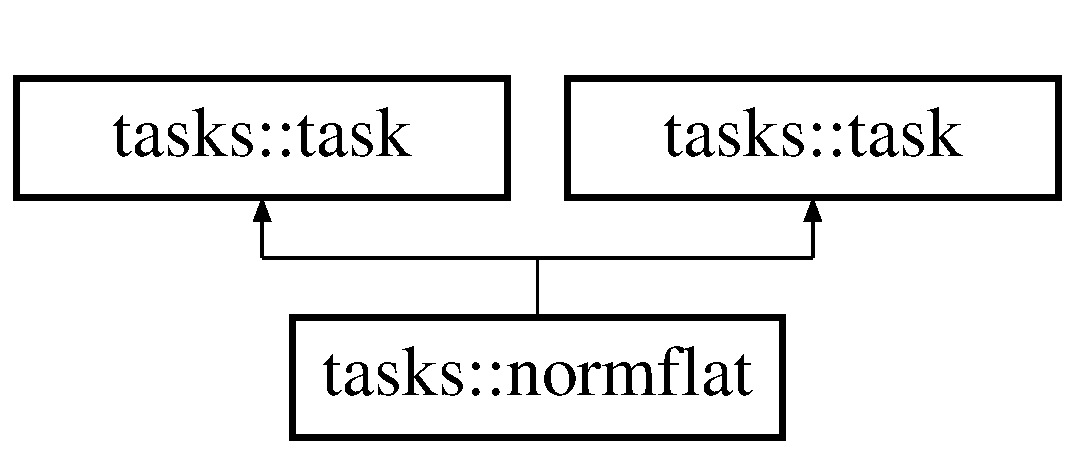
\includegraphics[height=2cm]{classtasks_1_1normflat}
\end{center}
\end{figure}
\subsection*{Public Member Functions}
\begin{CompactItemize}
\item 
def \textbf{run}\label{classtasks_1_1normflat_0455ac038859f5ae397c0ba9446b9568}

\item 
def \textbf{run}\label{classtasks_1_1normflat_0455ac038859f5ae397c0ba9446b9568}

\end{CompactItemize}
\subsection*{Static Public Attributes}
\begin{CompactItemize}
\item 
string \textbf{name} = '{\bfnormflat}'\label{classtasks_1_1normflat_cfd6c40c5390df753b56a52707f451b1}

\item 
string \textbf{button\-Text} = 'Create normal. comb. FLAT'\label{classtasks_1_1normflat_5720cd427cb5d721d24b81319f2cb9ea}

\item 
list \textbf{prereq} = ['{\bfsumflat}', '{\bffindord}']\label{classtasks_1_1normflat_57693ae545e00aab51aca37dd24b27f6}

\end{CompactItemize}


\subsection{Detailed Description}


\footnotesize\begin{verbatim}Calculate a 2D-normalized combined FLAT by fitting the 2-dimensional shape of the
   orders. The normalized combined FLAT can be used to correct for local changes in 
   responsivity of the CCD, for example fringes. In addition to the normalized FLAT,
   a frame containing the fitted blaze shape is calculated. 
\end{verbatim}
\normalsize
 



The documentation for this class was generated from the following files:\begin{CompactItemize}
\item 
old/PANICtool-1.0/tasks.py\item 
old/tasks.py\end{CompactItemize}
